% Overview 
To solve the problem of performing efficient searchs on spatial data, 
Guttman proposed the \rbase-tree, which inspired a plethora of different 
variations. In Section~\ref{sec:rtrees} we describe the original \rbase-tree, 
and in Section~\ref{sec:variants} we discuss the \rstar-tree, the variant most 
commonly used as a baseline for the structures discussed in later sections.

\subsection{R-Trees}
\label{sec:rtrees}
In 1984, Guttman proposed the idea of modifying the B-tree structure to
use minimum bounding rectangles (MBR) as a method to restrict the search space
during a lookup for spatial data\cite{guttman84}. The data structure that 
resulted from Guttman's research was called the R-tree. R-trees are structured
similarly to B-trees except, instead of having separation values in each 
internal node that divide its subtrees, R-tree internal node entries 
correspond to MBRs that bound its descendents. 
Figure~\ref{fig:R-Tree_structure} shows the R-tree representation for the 
objects of Figure~\ref{fig:R-Tree_objects}. As we observe, the MBR of a 
particular node entry completely overlaps the MBRs of the entries of its child
and its child's children. Nodes correspond to disk pages and leaves point to 
database objects.

\begin{figure}[t]
	\begin{subfigure}{0.48\textwidth}
		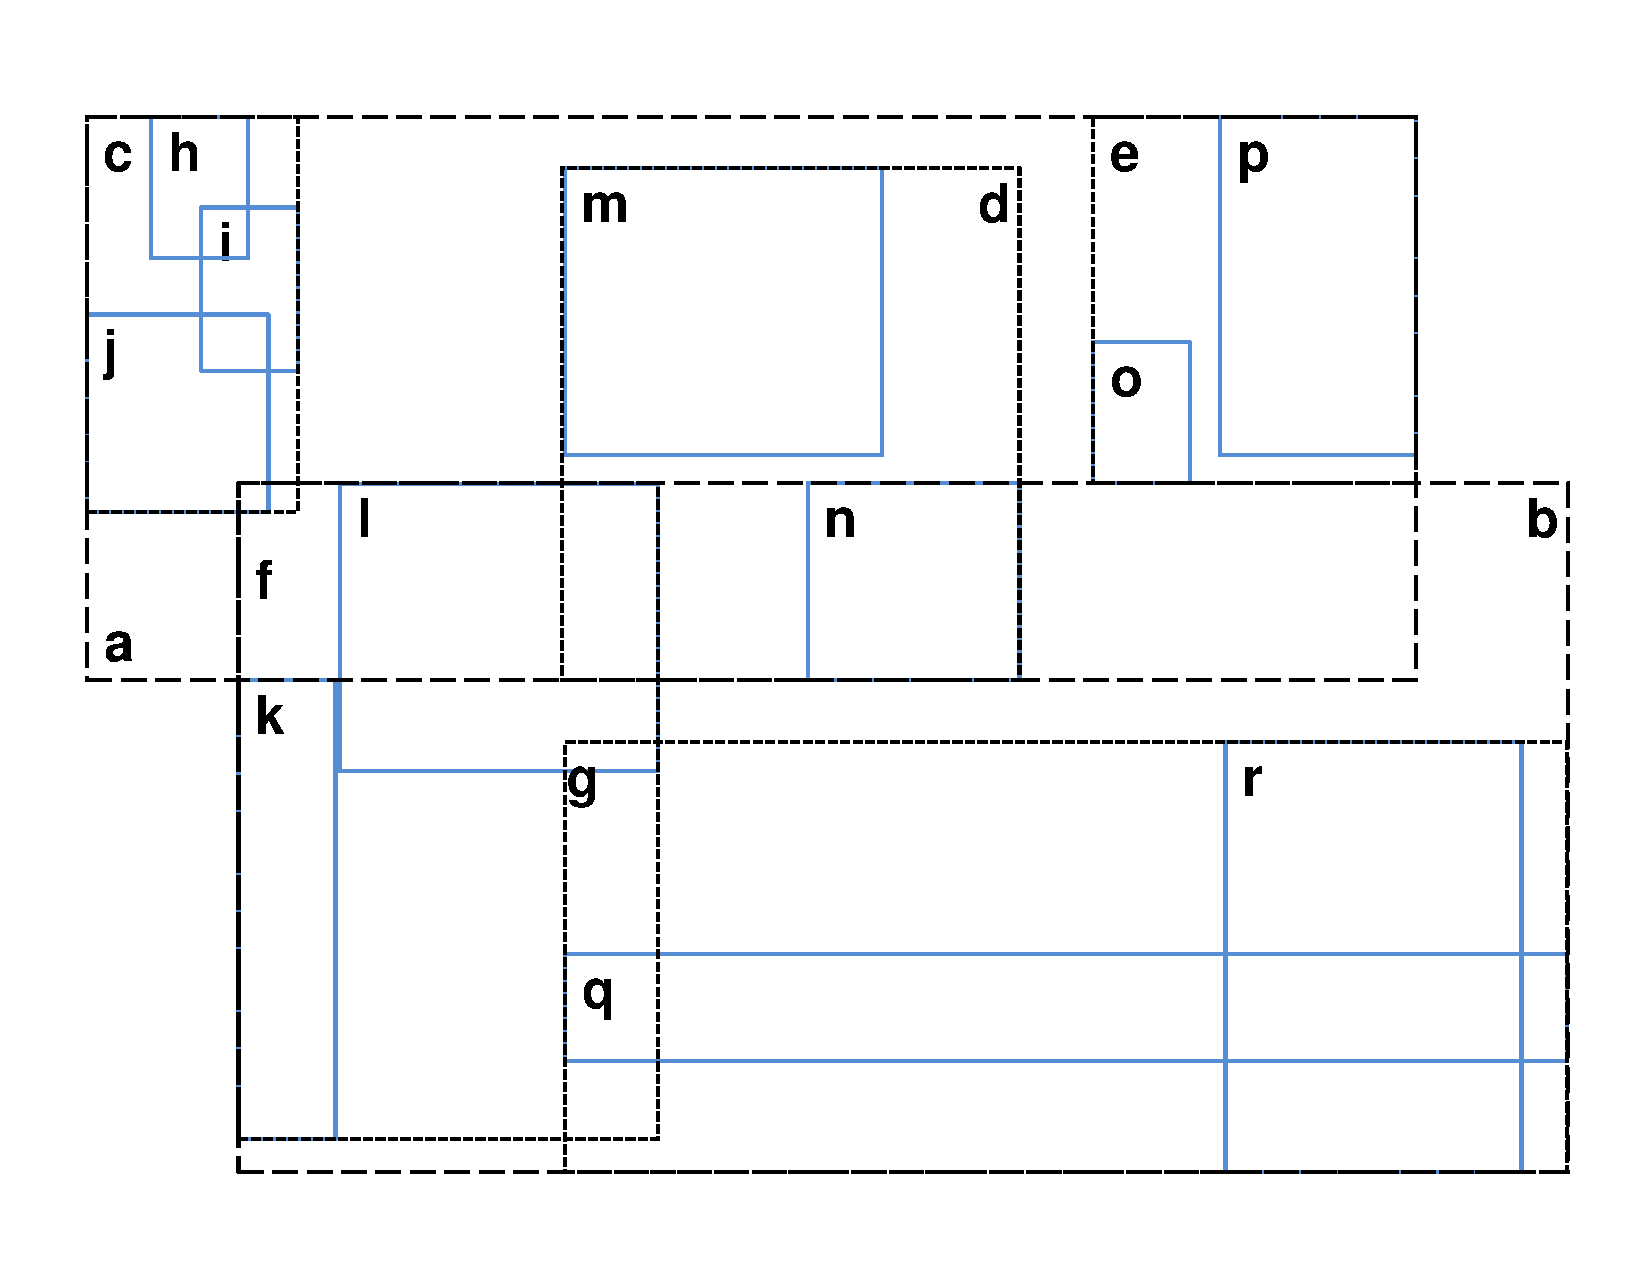
\includegraphics[width=\textwidth]{./figures/R_Tree_objects.pdf}
		\caption{Spatial objects bounded by MBRs}
		\label{fig:R-Tree_objects}
	\end{subfigure}
	~
	\begin{subfigure}{0.48\textwidth}
		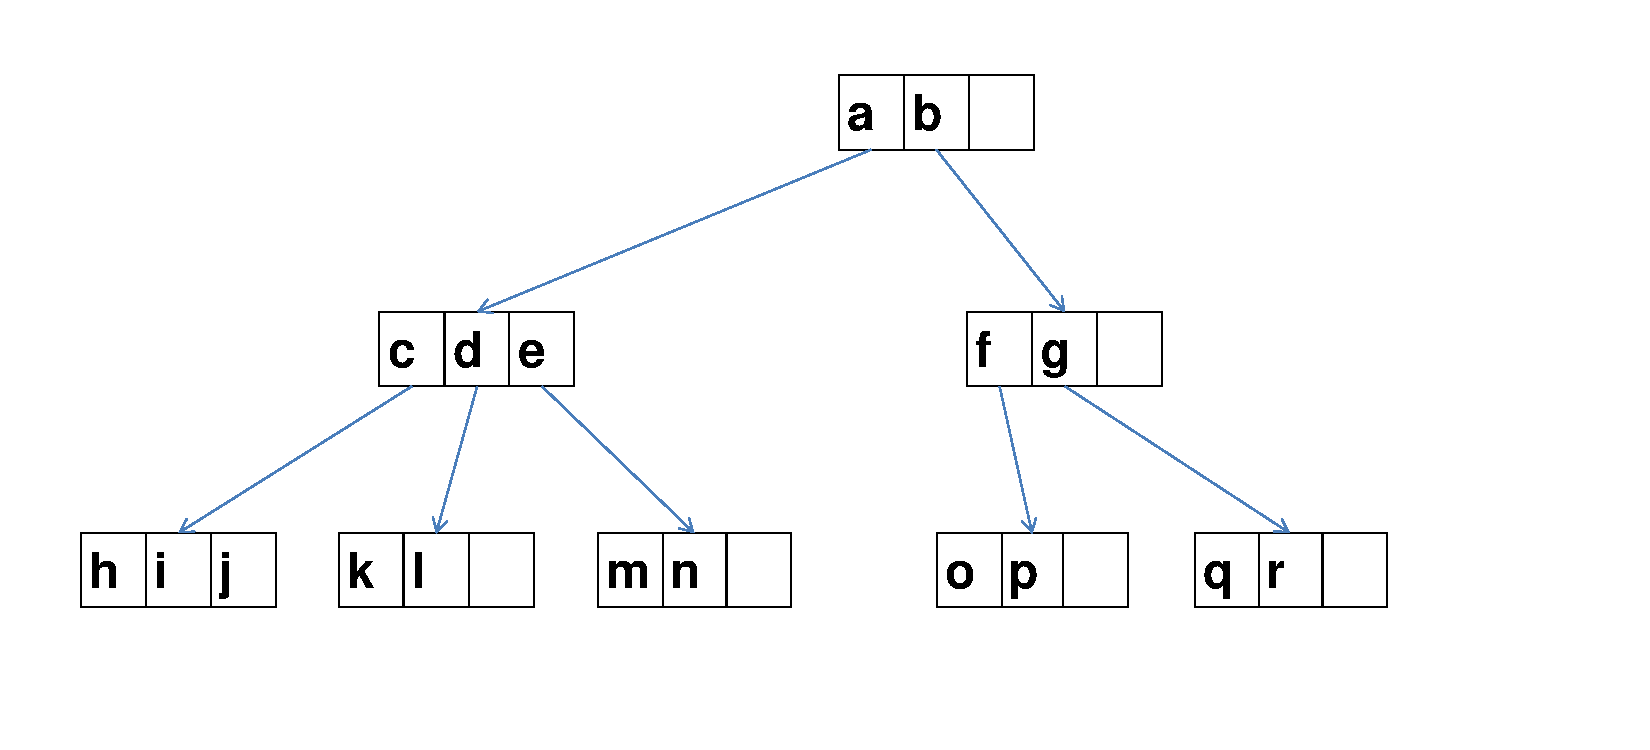
\includegraphics[width=\textwidth]{./figures/R_Tree_structure.pdf}
		\caption{R-tree structure for the objects of part a}
		\label{fig:R-Tree_structure}
	\end{subfigure}
	\caption{Spatial data and corresponding R-tree structure}
\end{figure}


R-trees are bound by two parameters $m$ and $M$, the minimum and maximum number
of entries for each node except the root, respectively. An internal node entry 
is of the form ($mbr$, $p$), where $mbr$ is the MBR containing the MBRs of its 
descendents and $p$ is the pointer to its child subtree. The $mbr$ entry is of 
the form ($I_{0}$, $I_{1}$, ..., $I_{n-1}$), where $n$ is the number of 
dimensions and $I_{i}$ is of form $[a$,$b]$, a closed bounded interval along 
the i-th dimension. Similarly, a leaf node entry is of the form ($mbr$, $oid$), 
where $mbr$ is the MBR containing the object, and oid is the identifier for the 
object in the database. Finally, the root node must have at least three entries
except if it is a leaf.

There are multiple operations that are associated with an R-tree, which we 
discuss in the following sections.

\subsubsection{Search and Update}
In order to find all entries overlapped by a bounding rectangle $S$ in the 
R-tree, the pseudocode of Figure~\ref{fig:R_Tree_Search} is used. In a similar 
fashion to a B-tree traversal, each node in the tree starting from the root is 
checked for overlap using the $mbr$ field in the entry. If there is overlap, 
the search descends into the subtree pointed to by $p$ until it reaches a leaf. 
If the leaf entry's $mbr$ overlaps with $S$, then the object ID $oid$ is 
returned. Note that there is no worst-case performance guarantee for this
algorithm.

Updates are slightly more complex. If a tuple is changed such that the MBR
covering it is also changed, its record in the R-tree must be deleted and then
reinserted. This makes the cost of an update relatively expensive.

\begin{figure}[t]
\begin{algorithmic}
	\Function{Search}{$T$, $S$}
		\If{$T$ is not a leaf}
			\ForAll{$E$ in $T$}
				\If{$E.mbr$ overlaps $S$}
					\State \Call{Search}{$E.p$, $S$}
				\EndIf
			\EndFor
		\Else
			\ForAll{$E$ in $T$}
				\If{$E.mbr$ overlaps $S$}
					\Return $E.oid$
				\EndIf
			\EndFor
		\EndIf
	\EndFunction
\end{algorithmic}
\caption{Pseudocode for finding all entries in a R-tree rooted at T overlapped 
	by a search rectangle S}
\label{fig:R_Tree_Search}
\end{figure}

\subsubsection{Insert}
Insertion again is similar to B-tree insertion methods, as illustrated by the 
algorithm in Figure~\ref{fig:R_Tree_Insert}. The algorithm traverses the tree 
to find the appropriate node to insert into and performs splits when inserting
into full nodes, but there is one important distinction: node splitting 
heuristics. B-tree node splitting is simple since it is only necessary to 
partition the two resulting nodes into two equally sized nodes. In R-trees, the 
goal typically is to create two nodes such that it is unlikely for both to be
examined on subsequent searches by minimizing the total area of the MBRs for
both nodes.

In the original R-tree paper, Guttman discusses three different types of node 
splitting algorithms of different complexities: linear, quadratic, and 
exponential. The linear split algorithm is the most lightweight, but may
result in suboptimal splits since it does not perform an exhaustive search on
all possible groupings. It divides a group of entries into two groups by first 
selecting two seed entries to be the first entries in each group. The two 
entries with the highest normalized separation along any dimension are chosen.
Of the remaining entries, a random one is chosen and placed in the group that 
would have the least enlargement. The exception is if the number of remaining 
entries plus the number of entries in one group is equal to $m$, the minimum 
number of entries in a node, all remaining entries are put into that group. 

The quadratic split algorithm is identical to the linear algorithm, except the 
entries chosen to be seeds are the ones with that have the most wasted space
if grouped together; in other words, the two entries that have the maximum $d$
where $d = area(MBR_{i,j}) - area(E_{i}) - area(E_{j}) $.
Also, the way the remaining entries are added is different than the linear 
algorithm. In this case, the area increase for both groups is calculated for each
entry, and the entry with the maximum difference between the two will be inserted 
into the group that will result in less enlargement.

The exponential split algorithm is an exhaustive search that enumerates all possible
groupings for the entries. Given an R-tree with $M$, the maximum number of entries
in a node, the search space for this algorithm is on the order of $2^{M-1}$.

\begin{figure}[t]
\begin{algorithmic}
	\Function{Insert}{$T$, $E$}
		\State \Call{ChooseLeaf}{$T$, $E$}
		\Comment{Traverse tree from $T$ to appropriate leaf.
			At each level choose node $L$ whose MBR will
			need the least enlargement to cover E.mbr or
			if there is a tie, choose node with minimum
			area. Return $L$
		}
		\If{$L$ is not full}
			\State Insert $E$ into $L$
		\Else
			\State \Call{SplitNode}{$L$}
			\Comment{Returns $L$ and $LL$ containing $E$ and the old
				entries of $L$}
		\EndIf
		\State \Call{AdjustTree}{$L$}
		\Comment{Ascend from leaf node $L$ up to the root $T$
			and propagate splits. }
	\EndFunction
\end{algorithmic}
\caption{Pseudocode for inserting into an R-tree rooted at T given an entry E}
\label{fig:R_Tree_Insert}
\end{figure}

\subsubsection{Delete}
Deletion is handled by the algorithm of Figure~\ref{fig:R_Tree_Delete}. First,
we find the leaf containing the entry to be deleted. Then, we handle the case
where nodes are underfull by calling $CondenseTree$ on the leaf that held
the entry. Instead of merging the underfull node with a sibling like in a 
B-tree, the node is deleted, the other nodes in the leaf are reinserted into 
the R-tree, and the ancestor MBRs are adjusted accordingly. Guttman argues that
reinsertion has two advantages; first, it is easier to implement, and second, 
it prevents deterioration of the R-tree. We will see in other implementations
of the R-tree that this is not the only strategy for deletion.

\begin{figure}[t]
\begin{algorithmic}
\Function{Delete}{$T$, $E$}
	\State \Call{FindLeaf}{$T$, $E$}
	\Comment{Traverse tree from $T$ to appropriate leaf.
			Return node $L$ containing $E$}
	\State Delete $E$ from $L$
	\State \Call{CondenseTree}{$L$}
	\Comment{Given leaf $L$ where $E$ was deleted, if $L$ was
	underfull, reinsert other entries in $L$, delete, and propagate changes
	upward}
\EndFunction
\end{algorithmic}
\caption{Pseudocode for deleting an entry E from an R-tree rooted at T}
\label{fig:R_Tree_Delete}
\end{figure}


%%%%%%%%%%%%%%%%%%%%%%%%%%%%%%%%%%%%%%%%%%%%%%%%%%%%%%%%%%%%%%%%%%%%%%%%%%%%%%
\subsection{R-Trees In Practice: The \rstar-Tree}
\label{sec:variants}
In practice, Guttman's original R-tree is not typically used. Instead the 
\rstar-tree of \cite{beckmannkriegelschneiderseeger90} is the variant most 
commonly used as the baseline structure for R-tree variants. The 
\rstar-tree introduces four optimization criteria for the data structure. 
These are listed below:

\begin{description}
	\item[O1: Minimization of area covered by each MBR] Minimize the amount of 
		deadspace to reduce the number of paths traversed during a query.
	\item[O2: Minimization of overlap between MBRs] Reduce the overlap to decrease the
		number of paths traversed during a query, especially point queries.
	\item[O3: Minimization of MBR perimeters] Minimize the margin of the MBR to 
		improve queries using large quadratic search rectangles and have better 
		data structure packing.
	\item[O4: Maximization of storage utilization] Increase utilization of nodes to 
		have a tree of shorter height and thus shorter query paths.
\end{description}

\begin{figure}[ht!]
	\begin{algorithmic}
		\Function{ChooseLeaf}{$R$, $E$}
			\If {$R$ is a leaf}
				\Return $R$
			\Else
				\For{$N$ in $R$}
					\If {$N.ptr$ is a leaf}
						\State $Cost$ = Overlap Enlargement of inserting $E$ into $N.ptr$
					\Else
						\State $Cost$ = MBR Area Enlargement of inserting $E$ into $N.ptr$
					\EndIf
				\EndFor
				\State $minNode \Leftarrow$ node with the lowest cost
				\Call {ChooseLeaf}{$minNode$, $E$}
			\EndIf
		\EndFunction
	\end{algorithmic}
	\caption{Pseudocode for choosing which leaf to insert entry $E$ into, given a 
	\rstar-Tree rooted at $R$}
	\label{fig:R*-Tree_ChooseLeaf}
\end{figure}

\begin{figure}[ht!]
\begin{algorithmic}
	\Function{Split}{$N$, $E$}
		\State{Determine the axis to split on}
		\For{dimension $i \Leftarrow 1 \to n$}
			\State {Sort entries by lower value of the interval, then by the
				higher value. Partition the entries into two groups such
				that the kth distribution has the first (m-1)+k entries in
				group 1 and the rest in group 2.}
			\State {$S \Leftarrow$ sum of all margin values of the 
				distributions from above.  }
		\EndFor
		\State{Select axis $i$ with the minimum $S$}
		\State{Choose the distribution with the minimum overlap along axis $i$}
		\State{Distribute the entries into two groups accordingly}
	\EndFunction
\end{algorithmic}
\caption{Pseudocode for splitting a full node $N$ given entry $E$ to be inserted into 
	a \rstar-tree}
\label{fig:R*-Tree_Split}
\end{figure}

\begin{figure}[ht!]
\begin{algorithmic}
	\Function{Insert}{$R$, $E$}
		\State $L\Leftarrow$ \Call{ChooseSubtree}{$R$}
		\If {$L$ has $<$ $M$ entries}
			\State insert $E$ into $L$
		\Else
			\If {$L \neq$ root and no reinsert has been done on this level}
				\State \Call {ReInsert}{$L$}
				\Comment {Reinsert $f$ entries whose centroid is furthest
					from the node centroid}
			\Else
				\State \Call {Split}{$L$}
			\EndIf
		\EndIf
		\State Propagate changes upward
	\EndFunction
\end{algorithmic}
\caption{Pseudocode for inserting entry $E$ into a \rstar-tree rooted at $R$}
\label{fig:R*-Tree_Insert}
\end{figure}

% Search, Insert, Node Splitting, Delete
Thus, the insertion algorithm varies greatly from Guttman's algorithm in 
Figure~\ref{fig:R_Tree_Insert}, especially its method of choosing a leaf and performing a 
split. Search and deletion, however, is no different from the R-tree. In 
Figure~\ref{fig:R*-Tree_ChooseLeaf} we see that the algorithm selects the path using criteria
O1 when descending into non-leaf nodes and O2 when descending into a leaf. This means that
the path chosen results in the least MBR enlargement on internal nodes and the least 
amount of overlap among leaf MBRs. 

Similarly, node splitting also considers the optimization criteria in order to determine
the split criteria and the distribution of entries among the two groups. In 
\cite{beckmannkriegelschneiderseeger90}, the authors examine three cost functions: total area 
covered by the resultant MBRs, total margin of the resultant MBRs, and the overlapping area 
of the MBRs. Of the algorithms examined in \cite{beckmannkriegelschneiderseeger90}, the one in 
Figure~\ref{fig:R*-Tree_Split} has the best overall performance. In this node splitting 
function, the axis with that minimizes the margin value is chosen for the split. Then, the 
distribution with the least area overlap is chosen to distribute entries. Note there is 
non-trivial cost associated with enumerating the different distributions.

We see in Figure~\ref{fig:R*-Tree_Insert} that leaf selection and node splitting are not
the only aspects that are different from Guttman's R-tree. We see that the insertion 
algorithm attempts to avoid splits by removing $f$ entries whose centroid distance from 
the node centroid is largest and reinserting them using $Insert$. 
 
The modifications on the $Insert$ algorithm have performance and utilization implications. 
For one, reinsertion causes decrease in overlap and better storage utilization. However,
its CPU cost is clearly higher than in R-trees, although the reduction of splits helps 
contain the I/O cost. In \cite{beckmannkriegelschneiderseeger90} we find that \rstar-trees 
outperforms the R-tree in terms of disk accesses and is not sensitive to skewed data distributions. 

% Is this necessary?
\subsection{Summary}
In summary, when Guttman introduced the R-tree it quickly became a popular structure
for spatial queries. Shortly after came the \rstar-tree, which was able to improve query 
performance and utilization of the R-tree by adding different insertion heuristics and 
optimization criteria. Thus the \rstar-tree is the base structure on which the variants 
in Section~\ref{sec:impchal} and Section~\ref{sec:dbchal} try to improve.
